\chapter{形状对齐的心室的分割方法}
\label{chap:Segmentation}
 
医学图像分割着重提取具有特殊含义的区域,如组织、肿瘤等,并使分割结果尽可能地接近解剖结构。进而辅助医生进行病情分析,诊断及制定治疗方案。如超声心动图可用于评估心室功能的各项参数,如左室容积、射血分数和行程容积等,其定量分析优于定性解释,特别是对于室壁运动和心室体积的估计。然而当前许多方法需指定初始输入,需要专家知识,如需手动勾勒短轴横截面,手动分析很耗时,也取决于观察者主观分析。自动或半自动分割算法是目前进行客观评价所必需的工具。目前虽已研究出各种分割方法,至今还没有一种能够统一适用于各种图像及不同部位的有效方法。由于解剖结构的个体差异较大,分割对象结构性质的千差万别;又由于噪声、伪影和容积效应等影响,使得己有分割算法远未达到理想效果。同时因无法完全用数学模型来简单描述所面临的实际问题;人们对分割结果预期目标互不相同等原因,只能针对特定问题和具体的需求,在精确度、鲁棒性和效率等关键指标上做出权衡\citep{Bosch2002}。

Hansson等\citep{Hansson2014}提出了贝叶斯概率图模型对心内膜概率进行建模分析,该方法使用左心室和心房相对位置的先验知识。基于能量泛函的活动轮廓及其扩展的水平集方法,如Marsousi等\citep{Marsousi2010}提出了一种,结合外力和采用多分辨率策略使用B样条自适应活动轮廓模型应用于超声心动图左心室心内膜分割。然而这些技术对初始化和参数选择非常敏感。在现有分割方法中,统计形变建模是用于可视化器官变化几何和功能模式的有效工具\citep{Santiago2016},典型建模的方法有可变形模板、点分布模型、图模型等。其分割是在有限的变化范围内进行的,变化范围通常由已知形状来定义。

统计形变模型是医学图像分割任务常用方法,其中表观建模又可分为全局和局部表观建模。
基于局部表观的主动形状模型(Active Shape Model,ASM)\citep{Cootes1995a} 和基于全局外观主动外观模型(Active Appearance Model,AAM)\citep{Cootes2001}用于超声心动图分割已被证明是非常有效的\citep{Bosch2002,Mitchell2002,Vargas-Quintero2016}。
原始ASM在超声图像中存在许多缺陷\citep{Santiago2016},因为它基于边缘灰度特征,也无法解决边缘缺失问题,局部受限模型\citep{Cristinacce2008a}(Constrained Local Model ,CLM)引入特征点局部区域外观模型加以改进。而AAM适合于2D和3D超声心动图中对左心室的复杂外观建模,因为它具有描述形状和图像强度的典型变化(包括伪影)的能力\citep{VanStralen2015}。

近来,级联形状回归模型\citep{Kazemi2014a}在特征点定位任务上取得较大突破,该方法使用回归模型,直接学习从表观到形状(或者形状模型的参数)的映射函数,进而建立从表观到形状的对应关系。此类方法不需要复杂的形状和表观建模,简单高效,在可控场景和非可控场景均取得不错的对齐效果。此外,基于深度学习的特征点定位方法\citep{Trigeorgis2016}也取得令人瞩目的结果。深度卷积神经网络结合形状回归框架可以进一步提升定位精度。但是基于级联形状回归和深度学习方法一般需要的数据量较大,不能直接适用于医学图像分割场景。

现有心室分割方法很少考虑心室的检测问题\citep{jixianghu-2016},默认操作是将平均形状手动放置于感兴趣区域,这导致最后的分割结果受初始位置影响较大。针对以上问题,我们提出一种基于沙漏卷积网络特征的多尺度形状对齐方法应用于超声心动图的左心室分割,在几个量化评价标准上的结果表明我们方法的有效性。

本工作提出的主要贡献如下:

1)初始化阶段,提出利用物体检测算法准确检测左心室位置,为后续分割自动化放置初始轮廓提供辅助,并构造心室分割数据库以评价算法,且针对训练深度卷积网络提出了扩充数据样本的方法。

2)提出利用全卷积神经网络学习外观和局部特征,构造多级沙漏卷积网络自动提取的特征融合了多种注意力图的上下文信息,实验详细比较了不同特征激活图的分割效果,在超声心动图心室分割任务上验证了基于深度学习的方法优于传统手工设计的特征。

3)综合分析了多种特征外观纹理和多种特征激活图,并克服AAM和CLM算法的缺点,利用各自的概率解释去统一全局AAM和局部CLM算法,得到最优的心室分割效果。

\begin{figure}[!htbp]
\centering
%trim option's parameter order: left bottom right top
%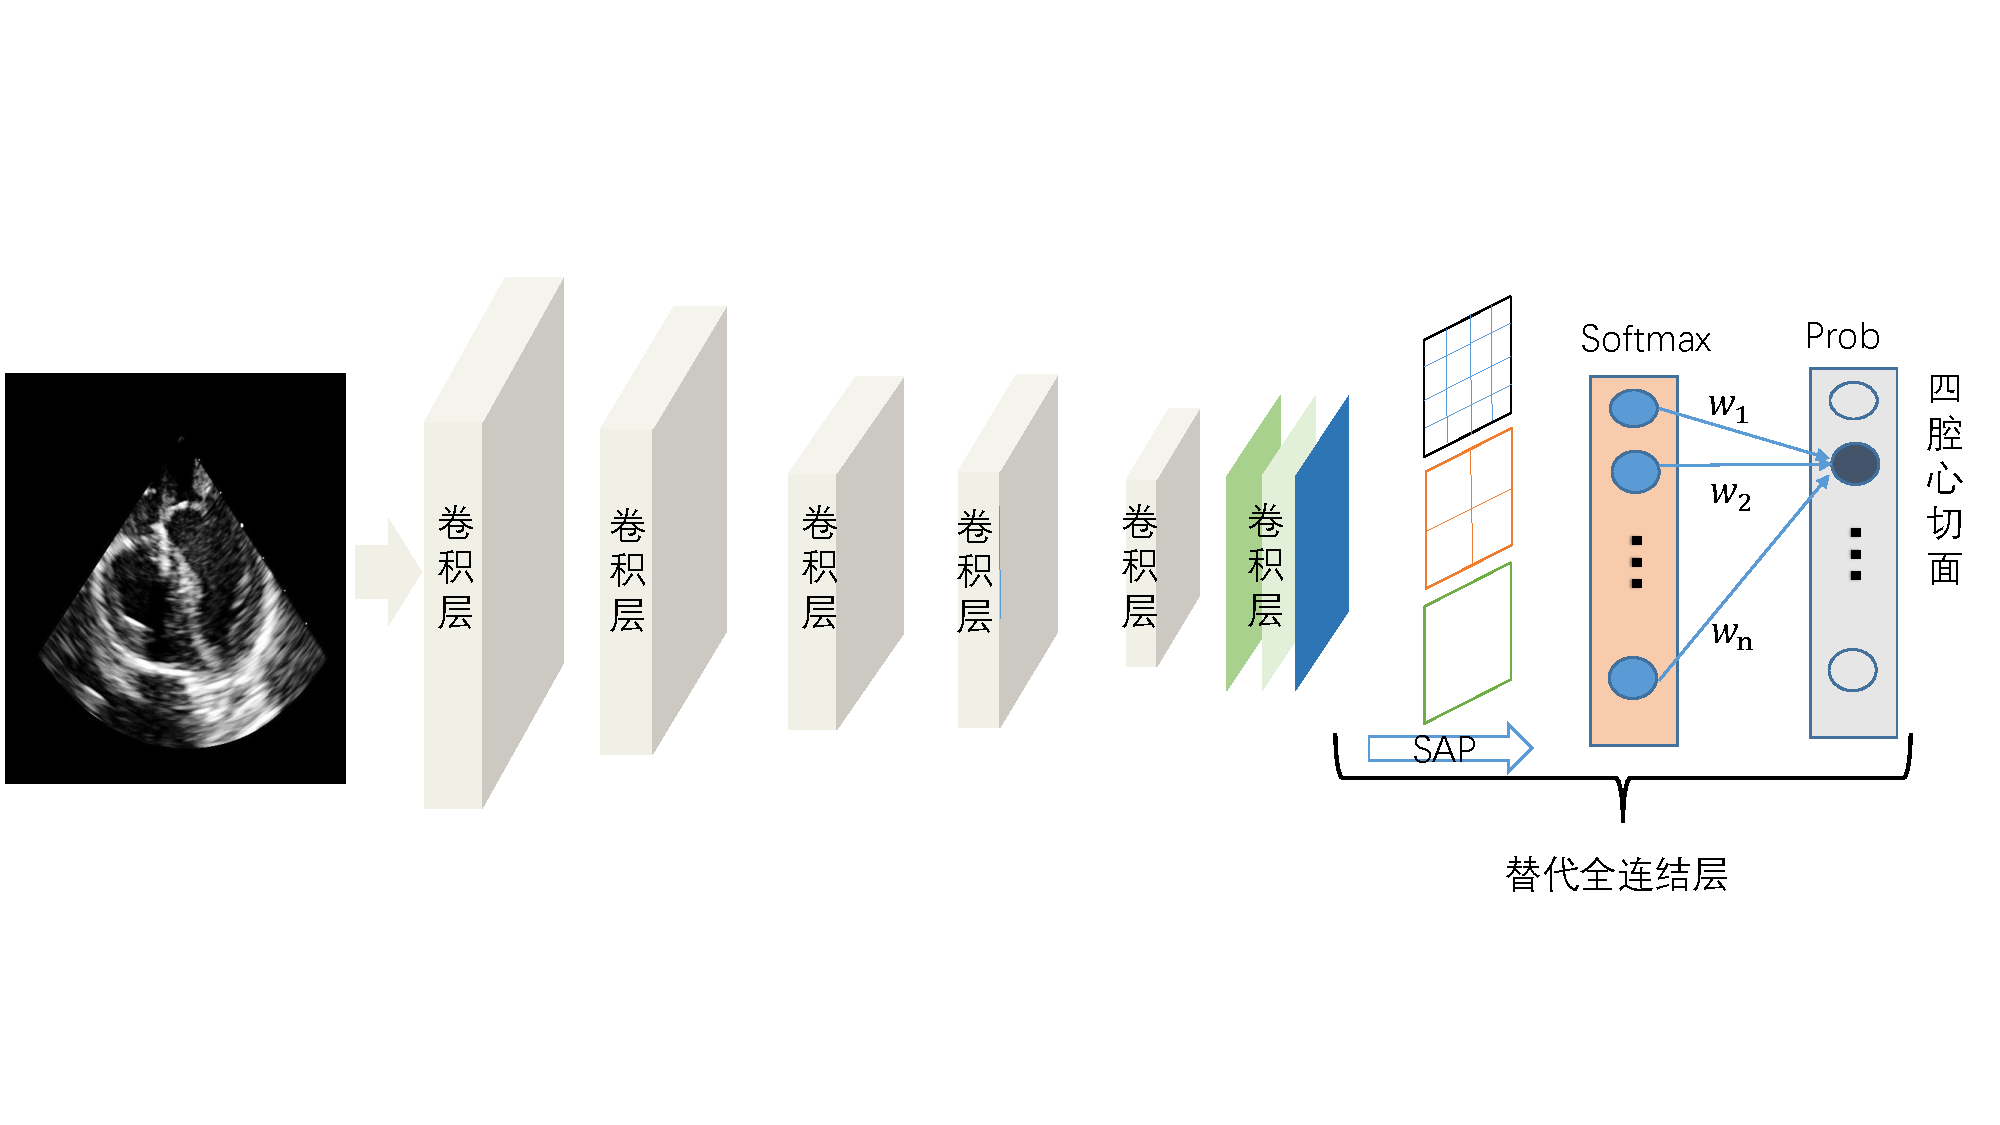
\includegraphics[trim = 30mm 0mm 30mm 0mm, clip, width=0.45\textwidth]{ch03_02}
\includegraphics[width=0.85\textwidth]{ch07_01}
\caption{初始位置定位结果和特征点标注示意图}
\label{fig:ch07_01}
\end{figure}
\section{初始位置定位和特征点标注}

检测左心室为下一步的分割和参数自动提取提供定位结果时,并未采用基于哈尔特征的稀疏积分图,结合提升回归分类器\citep{Zhou2007}和标注数据,将扫描窗口中外观映射为位移矢量, 学习回归函数的方法。
而是针对形变问题,基于图形结构的变形部件模型,使用梯度直方图(Histograms of Oriented Gradients, HOG)特征\citep{Dalal2005},结合线性支持向量机分类器和滑动窗口检测思想,对左心室进行检测。在实验数据上能100\%检测到左心室位置,检测结果如图\ref{fig:ch07_01}(a)所示,其中形变部件模板如图\ref{fig:ch07_02}(a)所示,能清晰看出内外膜轮廓。

 

斑点噪声和伪影的存在,使得难以定义一组生理上一致的特征点(不能表示相同的区域),从而难以构建有意义的统计表观模型。左心室特征点的标注同文献\citepns{jixianghu-2016}中一致,其中Centripetal Catmull-Rom曲线能够在减少特征点数量的同时得到形状一致的特征点,选用了34个特征点。如图\ref{fig:ch07_01}(b),外层曲线表示心外膜(0-16),内层曲线表示心内膜(0-16),图像的标注后的图像和生成纹理时的三角网格如图\ref{fig:ch07_01}(c)所示。

\begin{figure}[!htbp]
    \centering
    %trim option's parameter order: left bottom right top
    %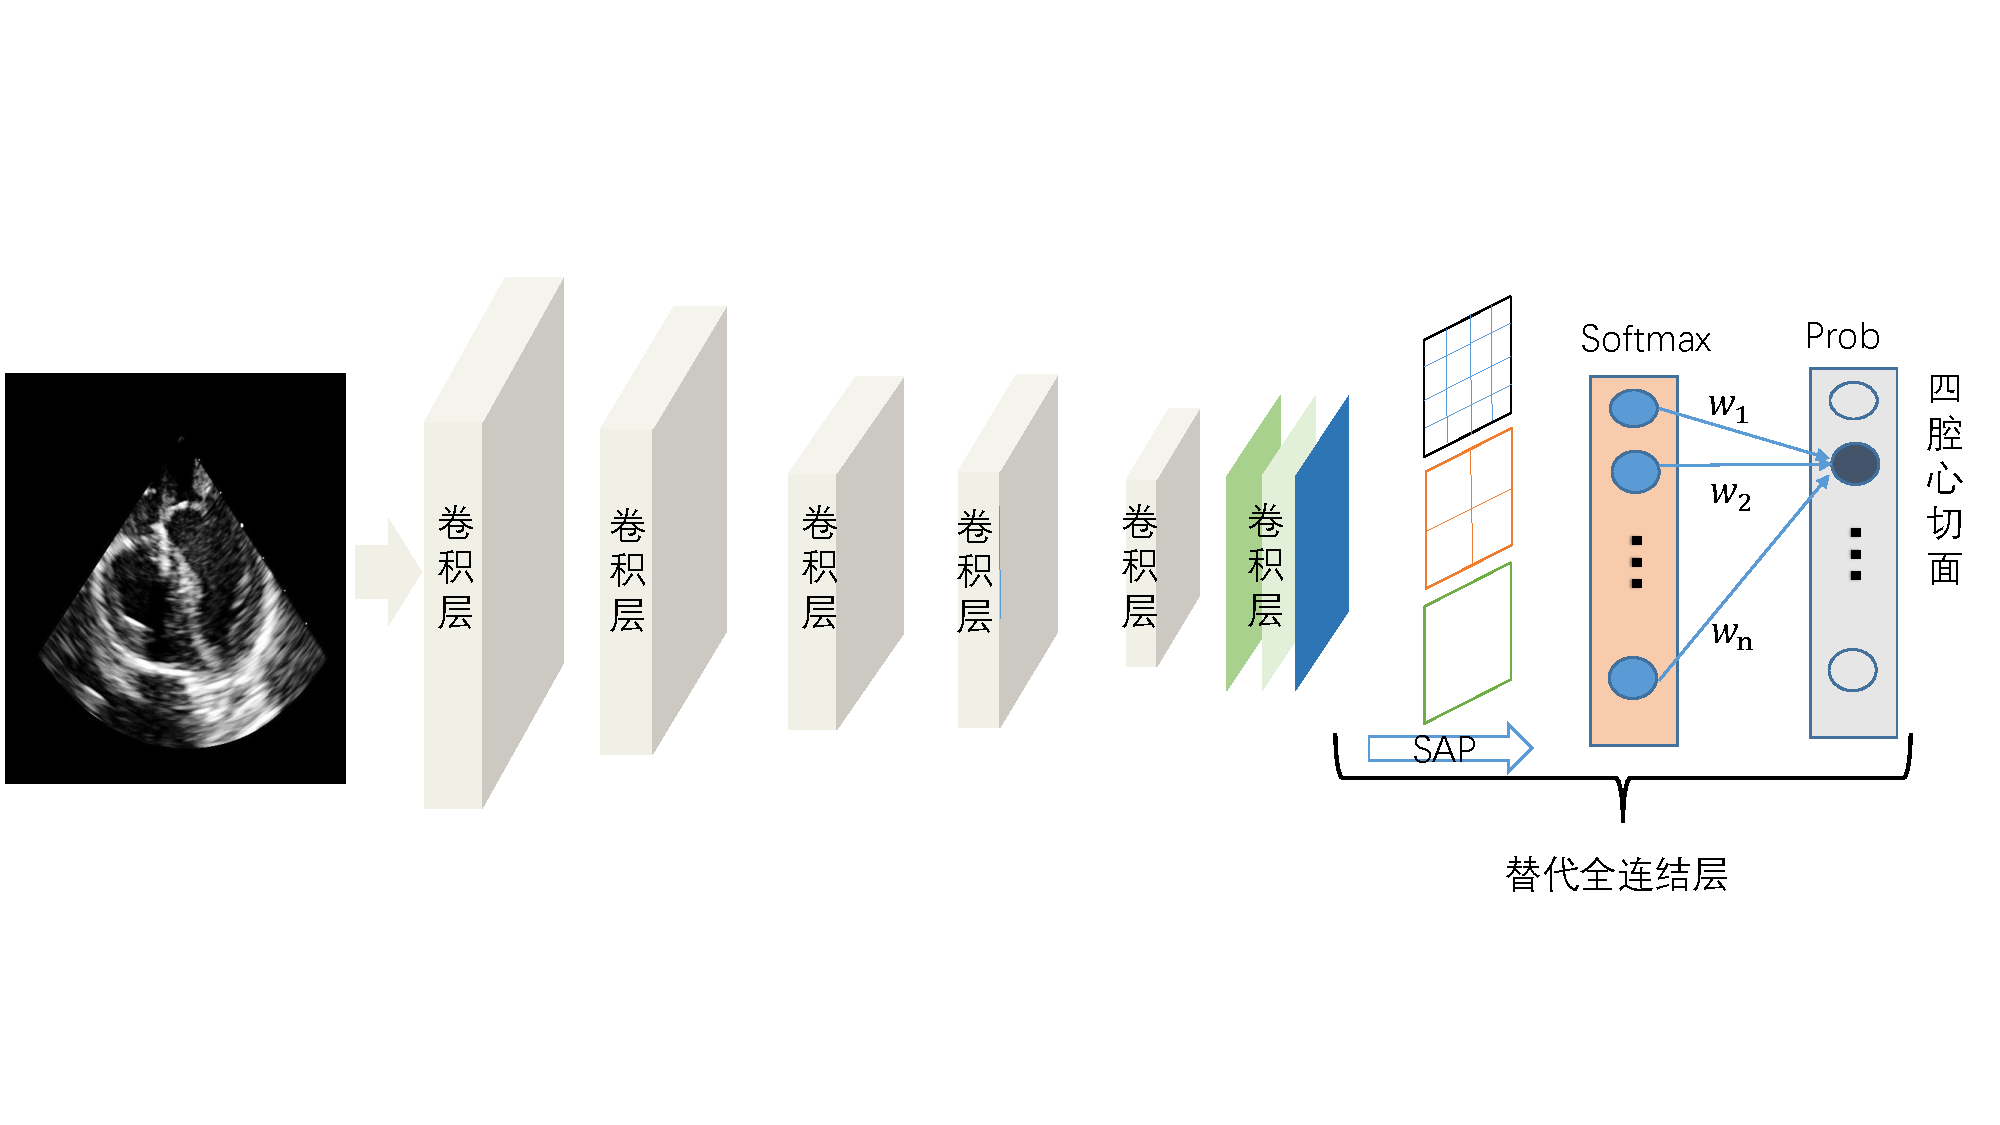
\includegraphics[trim = 30mm 0mm 30mm 0mm, clip, width=0.45\textwidth]{ch03_02}
    \includegraphics[width=0.85\textwidth]{ch07_02}
    \caption{定性比较三种不同特征激活图及相应的局部响应映射图, MCCF 通过多通道相关滤波器近似响应图,且用RLMS 算法移动到最优位置。SVR 基于支持向量机简单地选择最大响应位置。HG-n 表示所用不同HG 模块数的局部响应图,n 取1,2,4。}
    \label{fig:ch07_02}
    \end{figure}
     
\section{结合卷积网络特征的形状对齐模型} 

\subsection{超声组织特征纹理特异性灰度归一化} 
形状及外观模型利用PCA通过计算高维椭球分布的质心和主轴来模拟多维高斯分布。在标准AAM灰度归一化后,像素的灰度分布或多或少是高斯分布,使得平均灰度为0且方差为1。而超声心动图灰度直方图具有非高斯分布特征,直方图峰值处于非常低的灰度值,并且倾向于指数下降。这是超声图像的固有属性(尤其是斑点噪声),或多或少地独立于心室的组织类型,大致服从反指数分布或卡方分布\citep{Bosch2002},其宽度范围和偏移量变化很大,进一步的视频信号处理引入更多的偏移和增益变化,导致直方图峰值偏移,灰度范围可能会有很大差异。所以,在应用归一化之前,执行文献\citepns{Bosch2002}提出的非线性归一化来处理偏斜和偏移的灰度分布。

\subsection{结合不同外观特征的全局AAM}
全局AAM产生精确的拟合结果依赖于形状无关纹理的表示能力,对超声心动图使用图像灰度作为原始纹理来建立活动外观模型导致拟合不准确, 影响分割性能。同时标注数据困难,少量数据样本的外观变化较难建模,且心室腔体和腔壁有明显不同的纹理,提出可利用HOG特征、稠密SIFT特征以及后文提出的卷积网络特征,结合多尺度活动外观模型的左心室分割方法。不同特征的形状无关纹理直接影响AAM分割性能,图\ref{fig:ch07_02}表示采用灰度(图\ref{fig:ch07_02}(b)),hog特征(图\ref{fig:ch07_02}(c))构建的AAM模型的形状无关纹理可视化结果。AAM的参数空间的维度很大使得它们难以优化,此外还对不准确的初始化非常敏感。
\begin{figure}[!htbp]
\centering
%trim option's parameter order: left bottom right top
%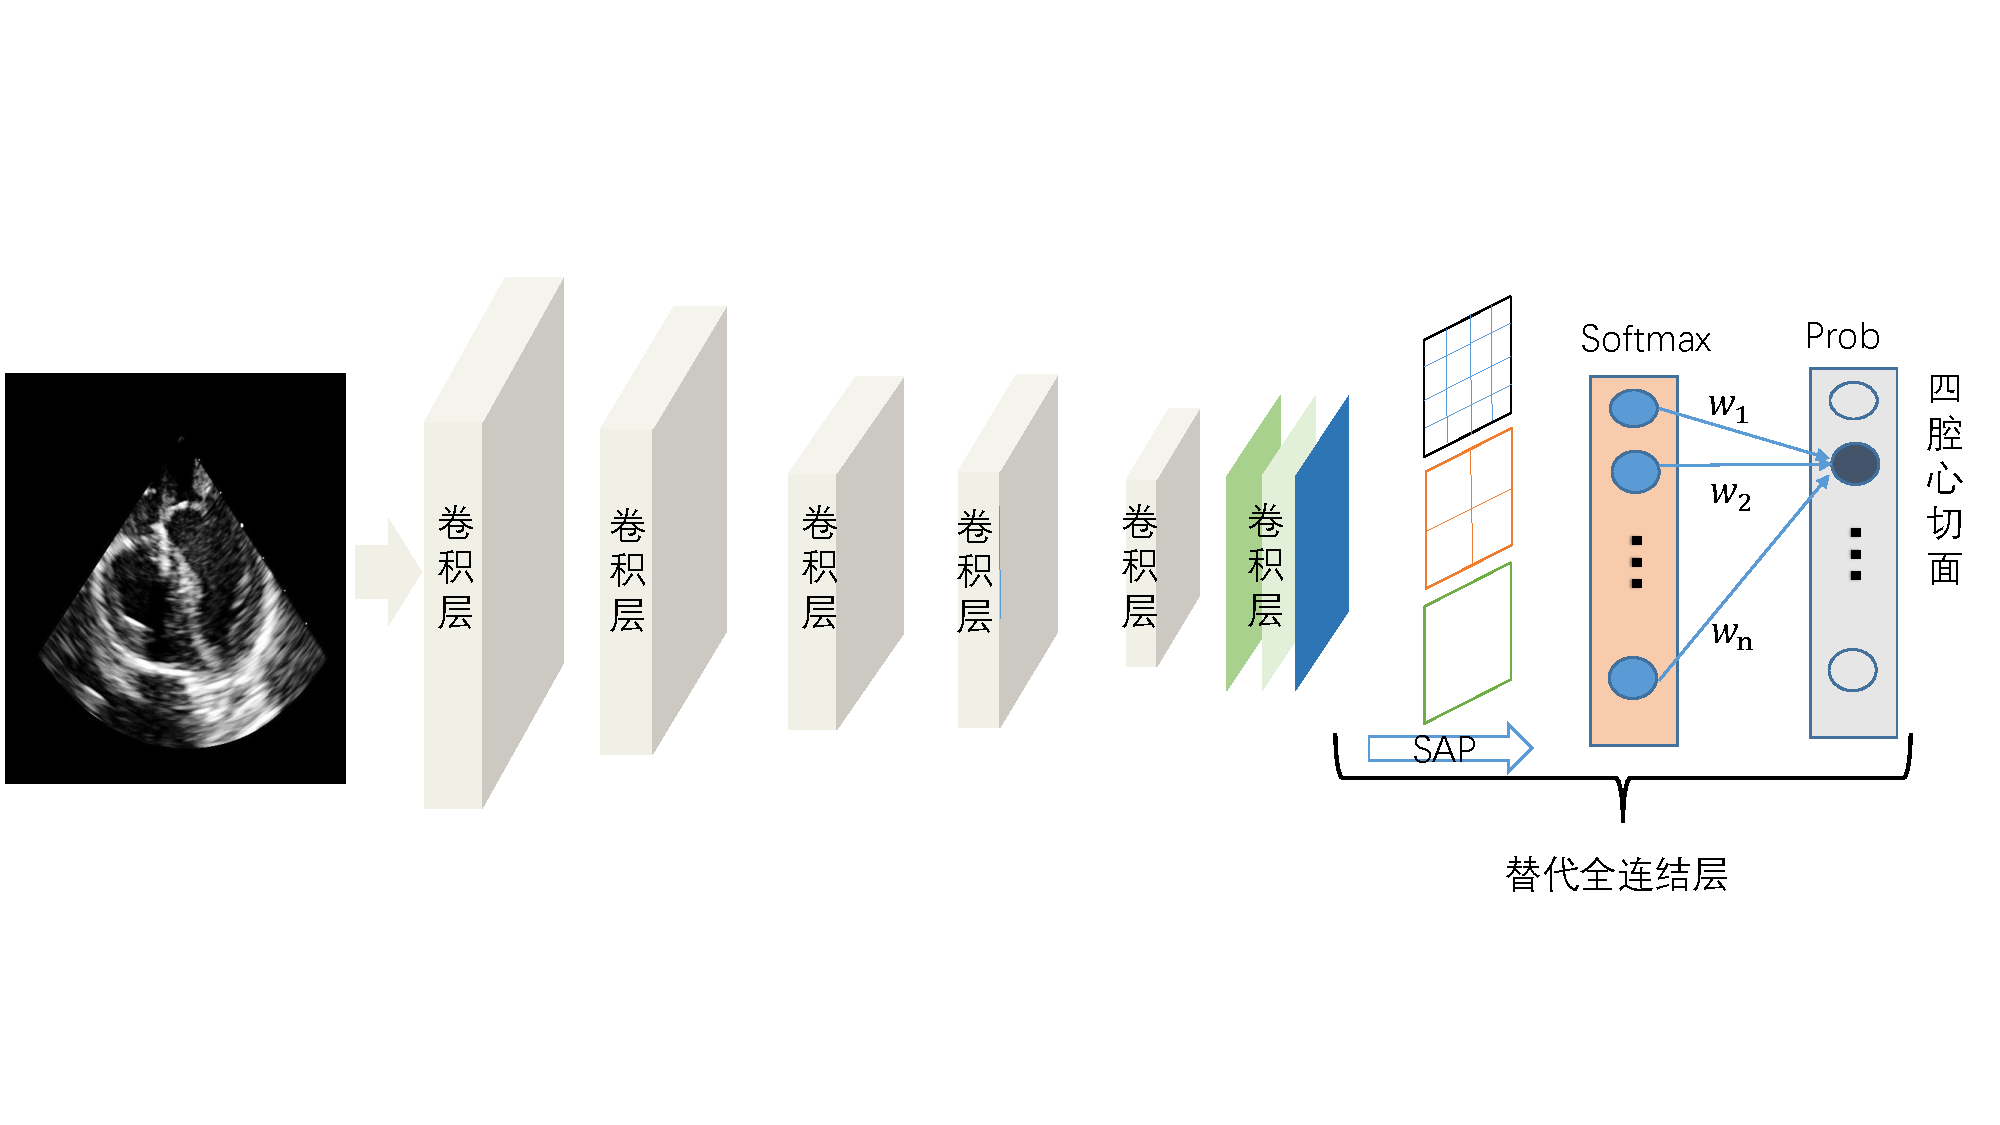
\includegraphics[trim = 30mm 0mm 30mm 0mm, clip, width=0.45\textwidth]{ch03_02}
\includegraphics[width=0.85\textwidth]{ch07_03}
\caption{不同特征的形状无关纹理图}
\label{fig:ch07_03}
\end{figure} 
 
\subsection{CLM中的特征激活图}
CLM算法最重要的一步是计算响应图,通过评估各个像素位置的标记点对齐概率,帮助准确地定位标记点。比较常用的多通道相关滤波(MCCF)\citep{Galoogahi2016}和支持向量回归机(SVR)\citep{Jan2017}的特征激活映射图可知,在超声心动图分割任务中,这些基于手工设计的特征效果差且不据有可解释性(见图\ref{fig:ch07_02})。在我们的模型中,这是由堆叠多级沙漏全卷积网络(Hourglass Network, HG)\citep{Newell2016a}完成的,围绕当前估计的所有标记点位置n×n像素区域作为感兴趣区域输入,并且输出在每个像素位置评估标记点概率响应图(见图\ref{fig:ch07_02}),网络结构如图\ref{fig:ch07_03}所示。 
\begin{figure}[!htbp]
\centering
%trim option's parameter order: left bottom right top
%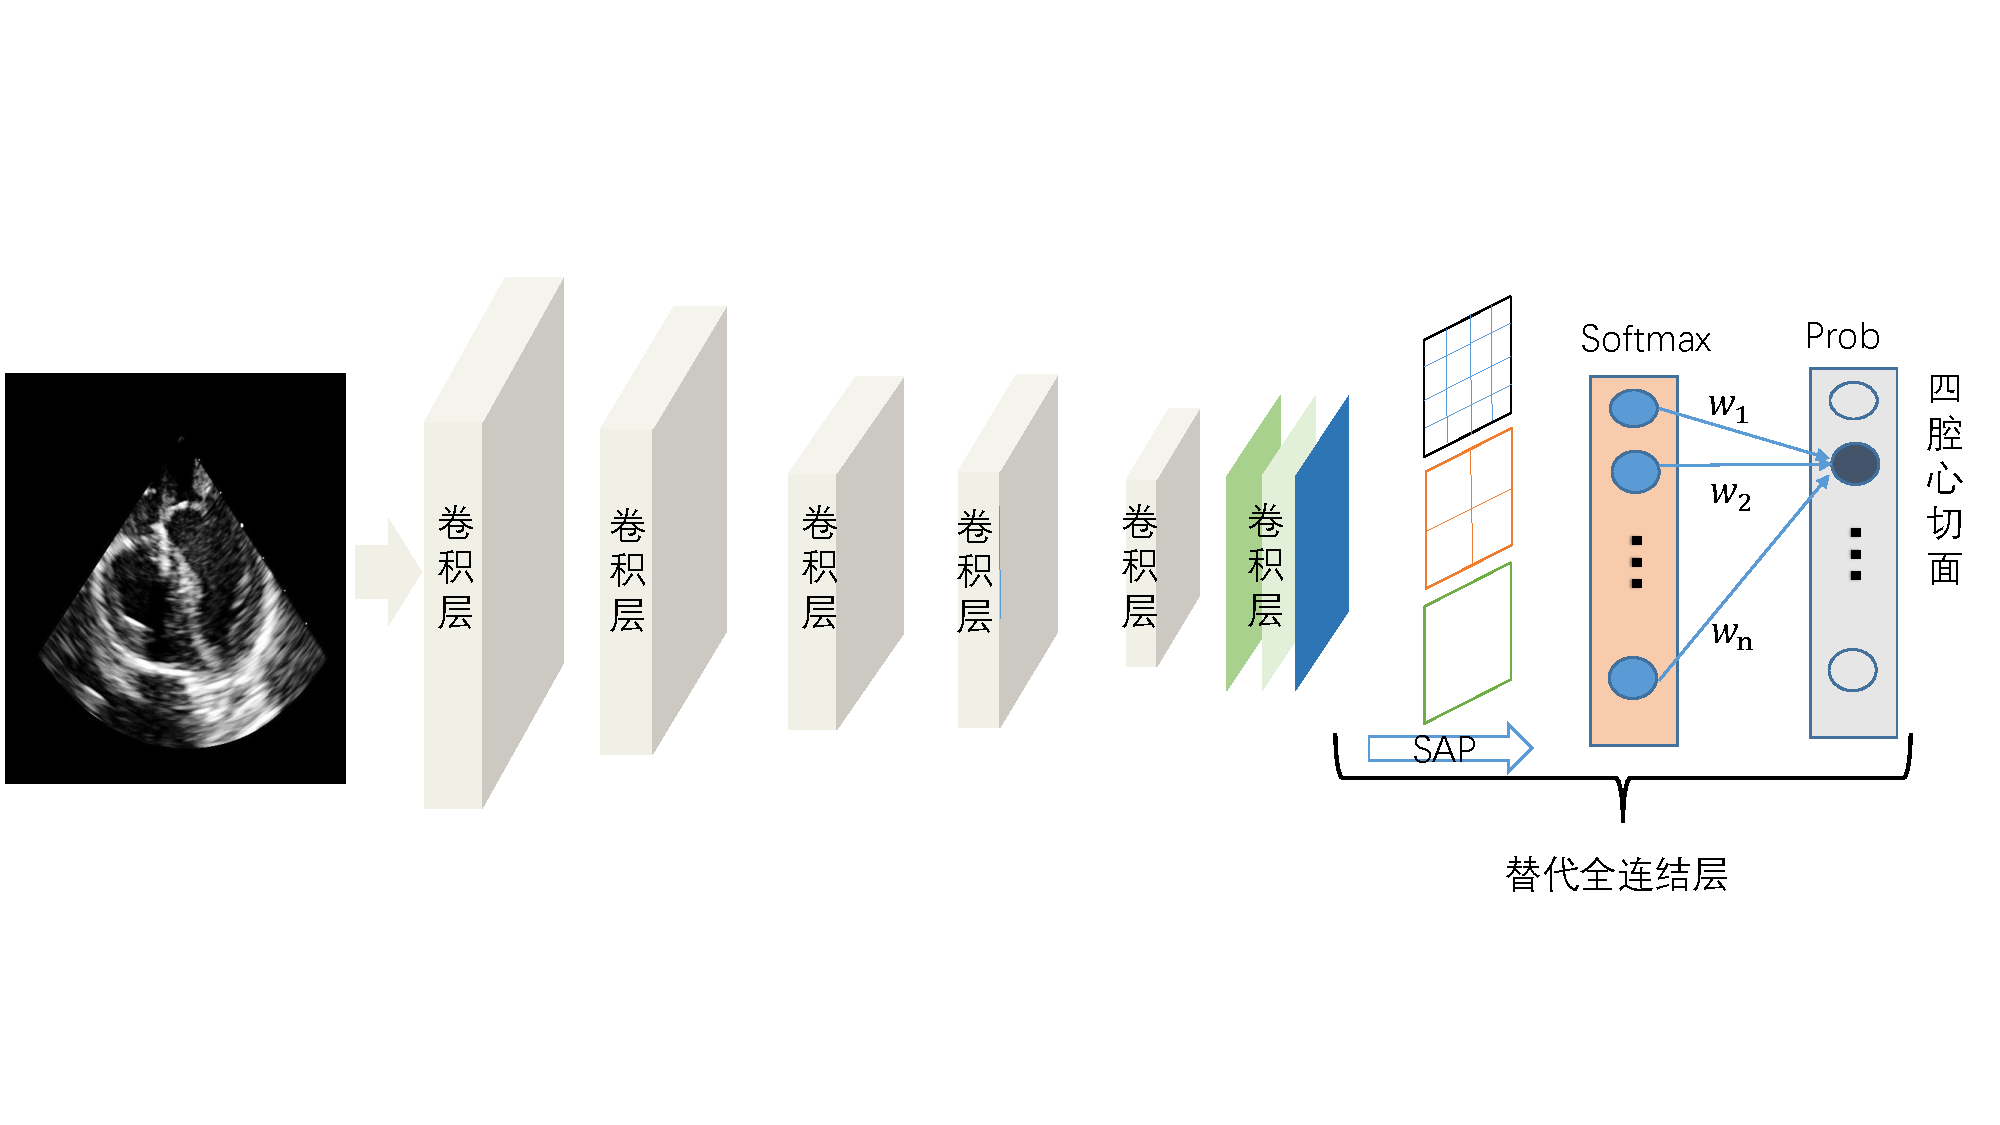
\includegraphics[trim = 30mm 0mm 30mm 0mm, clip, width=0.45\textwidth]{ch03_02}
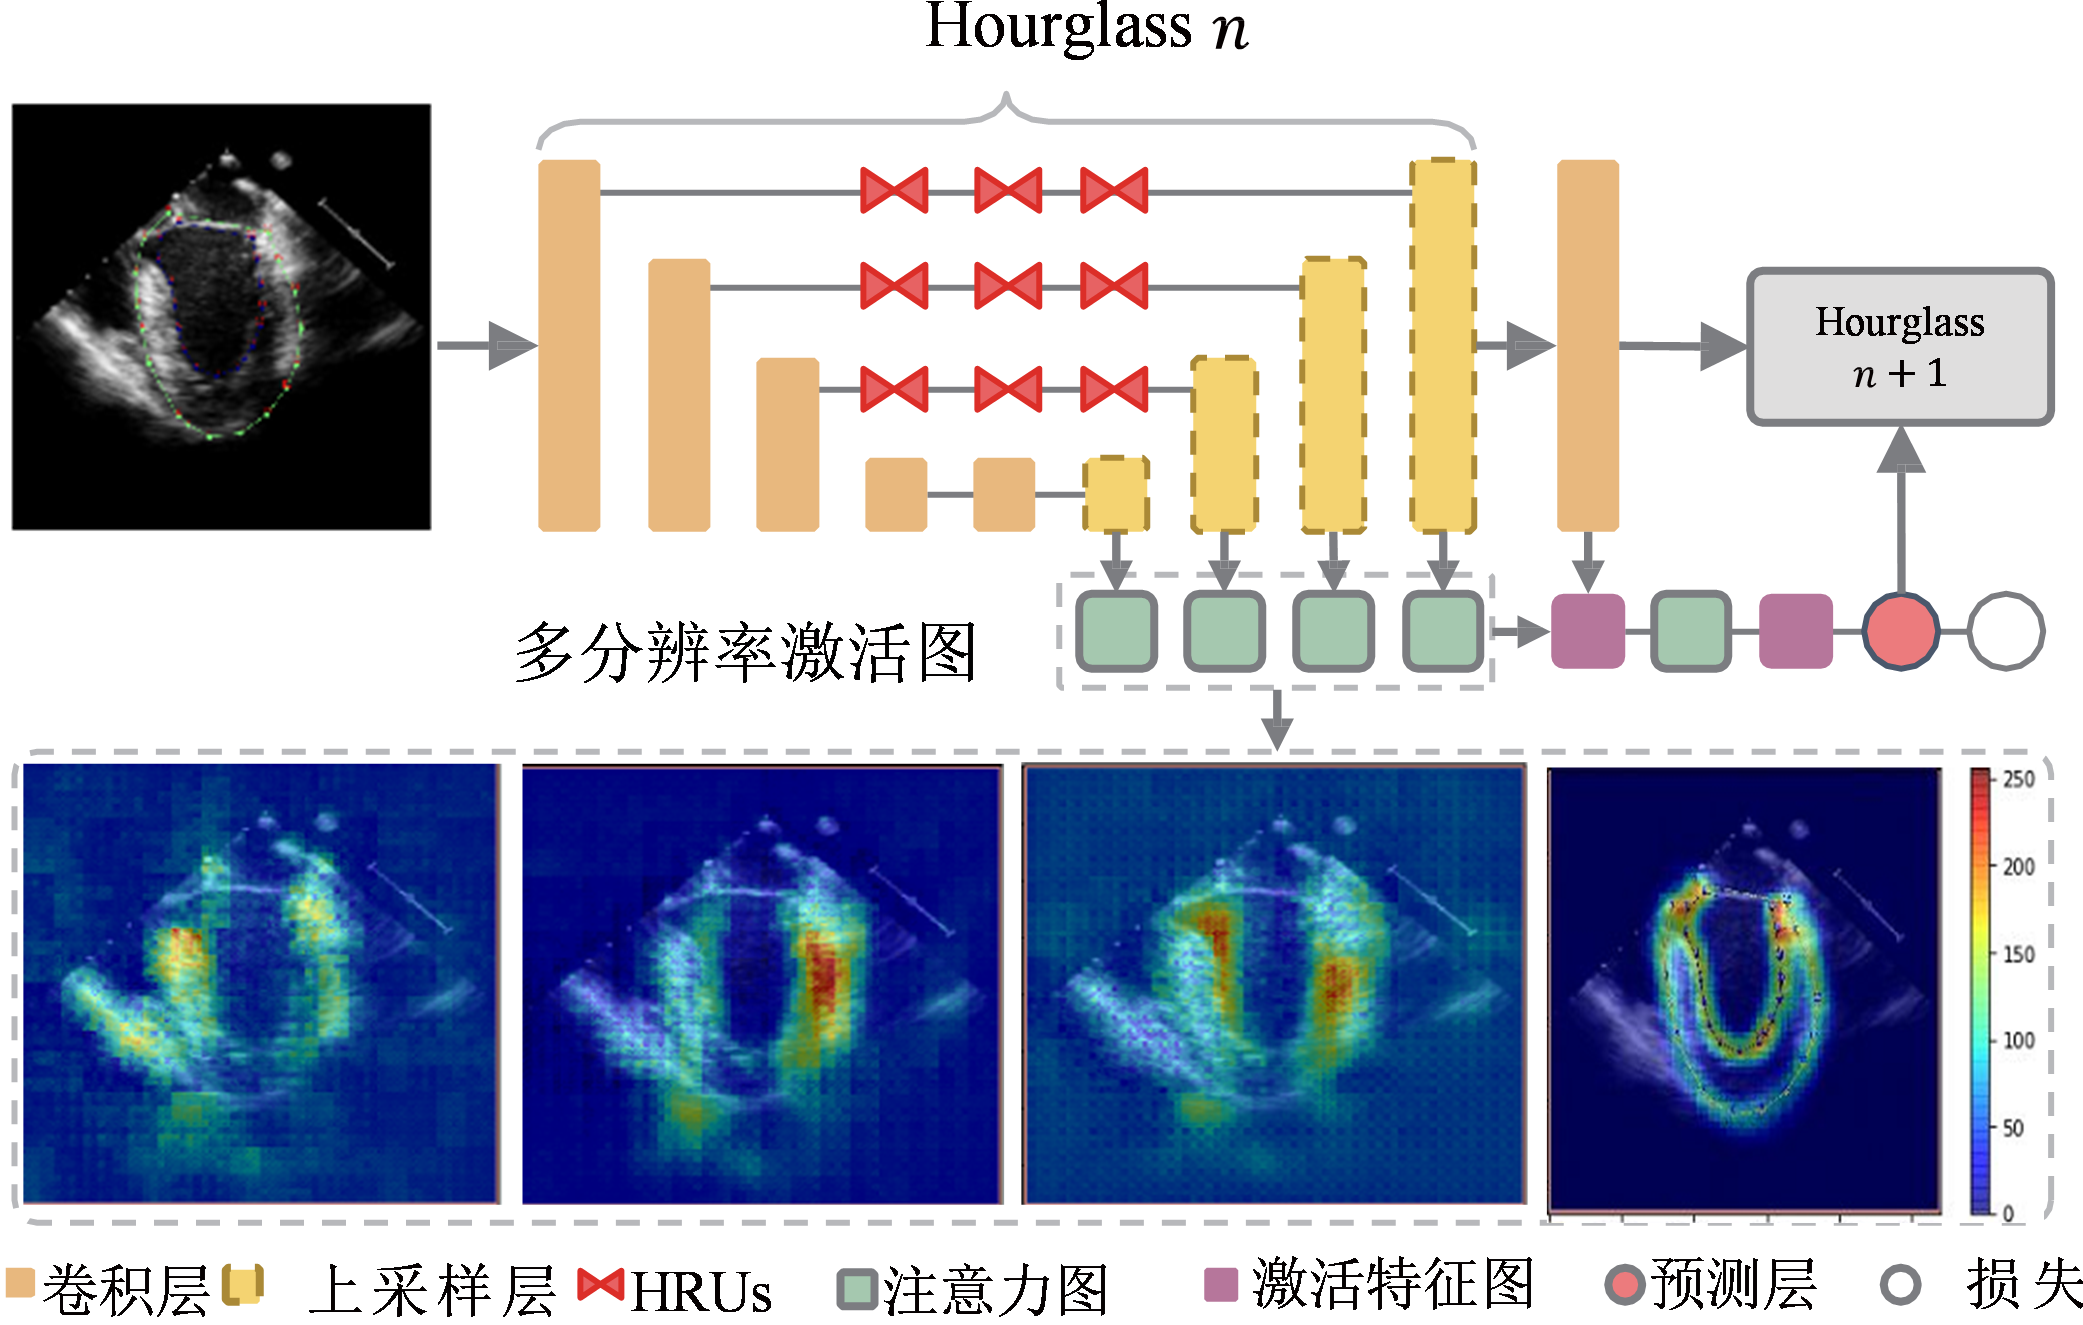
\includegraphics[width=0.85\textwidth]{ch07_04}
\caption{在每个沙漏网络中,从具有不同分辨率的特征生成多分辨率注意力图,这些图加和成单一的注意力图,它用于生成激活特征图。}
\label{fig:ch07_04}
\end{figure} 
 

图\ref{fig:ch07_03}中的网络基本组件是一种基于残差网络\citep{he15}。“沙漏”型网络结构是拓扑对称的,能够捕获和整合来自不同尺度和分辨率的信息。如图三中卷积层为残差模块,其是 3×3大小卷积核组成的卷积层、批归一化层和修正线性激活单元层来提取特征,同时用跳跃连接保留原始信息的统称。所有卷积层不改变数据尺寸,只改变通道数。在最大池化(max-pooling)下采样操作之前,它分离单个通路以将当前信息保留。在上采样(反卷积或最近邻插值)操作之前,添加与原始图像大小相同的特征图。在两次下采样操作的处理之间,为获得不同分辨率的注意力图\citep{Chu2017} ,同使用另一个残差模块提取来的特征图进行加权乘积得到激活特征图。对于H×W×3的输入图像,每一个HG级的激活特征图都会生成一个H/4×W/4×K的预测概率响应图,K表示标记点个数。对于每个响应图,都比较其与真值标记点附近高斯分布的欧式误差,作为损失函数中继监督(intermediate supervision)训练所有模块。详细的网络参数和训练过程在\ref{chap:Segmentation}4.1节中给出。
在公式10的迭代中,将感兴趣区域图像输入HG网络,输出了评估单个标记点对齐的概率响应图。将标记点i拟合到位置xi遵循以下等式: 
	  	(11)
式中li表示第i个标记点,图像的位置xi处的图像Ixi,响应映射πi用于最小化等式10。我们的消融实验实验表明,增加HG模块数,显著影响分割性能。

\subsection{统一AAM和CLM的概率解释}
整体和局部模型之间的差异在于提取外观向量以及构建变形模型的方式不同。基于整体或局部外观表示的选择高度依赖于建模对象及其内部结构的性质。针对医学图像分割问题,局部图像特征的位置并不总是对应于由专家人类观察者绘制的期望轮廓。因此,轮廓的确切位置不能总是从最强的概率响应图来确定,而是应该由专家观察者提供的示例建模学习得到。
为了结合全局和局部框架,采用一种可变形模型拟合问题的概率解释,式5和式10可以重写为以下优化问题:
    (12)
其中R(p,c)对应于复杂形状和纹理变形的正则化项,D(I,p,c)表示全局未对准度量,并对应于AAM拟合中的数据项, 表示对应于CLM拟合中数据项的v个标记点对齐的局部偏差度量。

\subsection{模型匹配代价函数的优化} 

等式12可以通过反向组合用于拟合AAM的梯度下降算法和用于拟合CLM的RLMS算法来优化,如结合投影反向组合(PIC)算法\citep{Jan2017}和RLMS算法,增量形状参数δp*的最优解由下式给出:

          (13)
          
其中:
	  	(14)
其中  是反向位置的海森矩阵(Hessian)。  和  分别是反向组合雅各比矩阵(Jacobian)和投影运算。或通过将交替反向组合(AIC)算法\citep{Jan2017}与RLMS组合:

 (15)
在这种情况下,Hessian和Jacobian被定义为  和  ,有关如何计算∂W/∂p的更多细节有兴趣的读者请参考\citep{Jan2017},最佳纹理参数c *由式5给出,且两种算法仍然使用式13定义的完全相同的更新规则得到δp*的最优值。

\section{实验结果分析和讨论}
\subsection{数据集增强和评价标准}

本实验采用Philips CX50和IE33所采集的带乳头肌和无乳头肌心脏四腔心经食道超声图像,共45个视频。专家标注(ground truth)由四川华西医院的麻醉科医生完成,其结果作为“金标准”。在训练过程中,我们用大致相同尺度的图像以心室为中心裁剪图像,并将图像缩放到256x256的大小作为输入。然后我们随机旋转、镜像翻转和缩放扩增数据集(包括图像和注释),其中需要注意的是要标注标记点有无的模版以应对标记点缺失的情况,最后扩增10倍获得4240个训练样本作为训练集,而167张的测试集不做任何数据扩充。
实验所有方法均使用前文提出的左心室检测算法估计轮廓初始位置。评价指标采用人脸对齐任务中常用的评价标准,使用平均点对点误差归一化欧式距离(NMSE):
	  	(16)
式中表示n个特征点的两个形状 和 ,lt和rb是真实形状边界的左上点和右下点的位置。归一化能够使性能测量与实际心室尺寸或缩放系数无关。本文采用NMSE的累积误差分布函数(Cumulative error distribution, CED)进行性能评估。同时计算两个形状之间的距离,然后统计测试集中所有形状与专家标注形状之间的距离的均值和方差。训练HG网络模型我们采用tensorflow框架,初始学习率为1×10-3,网络参数由Adam算法\citep{Kingma2014}优化,网络中开始是步长为2,核大小为7×7的卷积层,将分辨率由256降到64,以减少GPU占用,其后是残差模块和一串下采样层组成的HG模块,整个网络中的所有残差模块输出特征数都是256,相关代码见 。
本文实验采用三种方式:一是将比较不同特征的AAM和CLM,以验证使用单独全局和局部模型的最优分割效果;二是,在统一AAM和CLM的条件下,比较不同特征激活图对最终分割效果的影响;三是,在同样使用HG网络特征的条件下,将使用的HG模块数设为1、2、和4,比较不同数值下的分割效果。

\subsection{不同特征的AAM和CLM分割结果}
实验中,选取三个尺度的AAM模型,变形扭曲函数选择的是薄板样条曲线映射扭曲函数,平均形状作为参考形状获得形状无关纹理,优化算法统一为 PIC,每个尺度最大拟合30步。
\begin{figure}[!htbp]
\centering
%trim option's parameter order: left bottom right top
%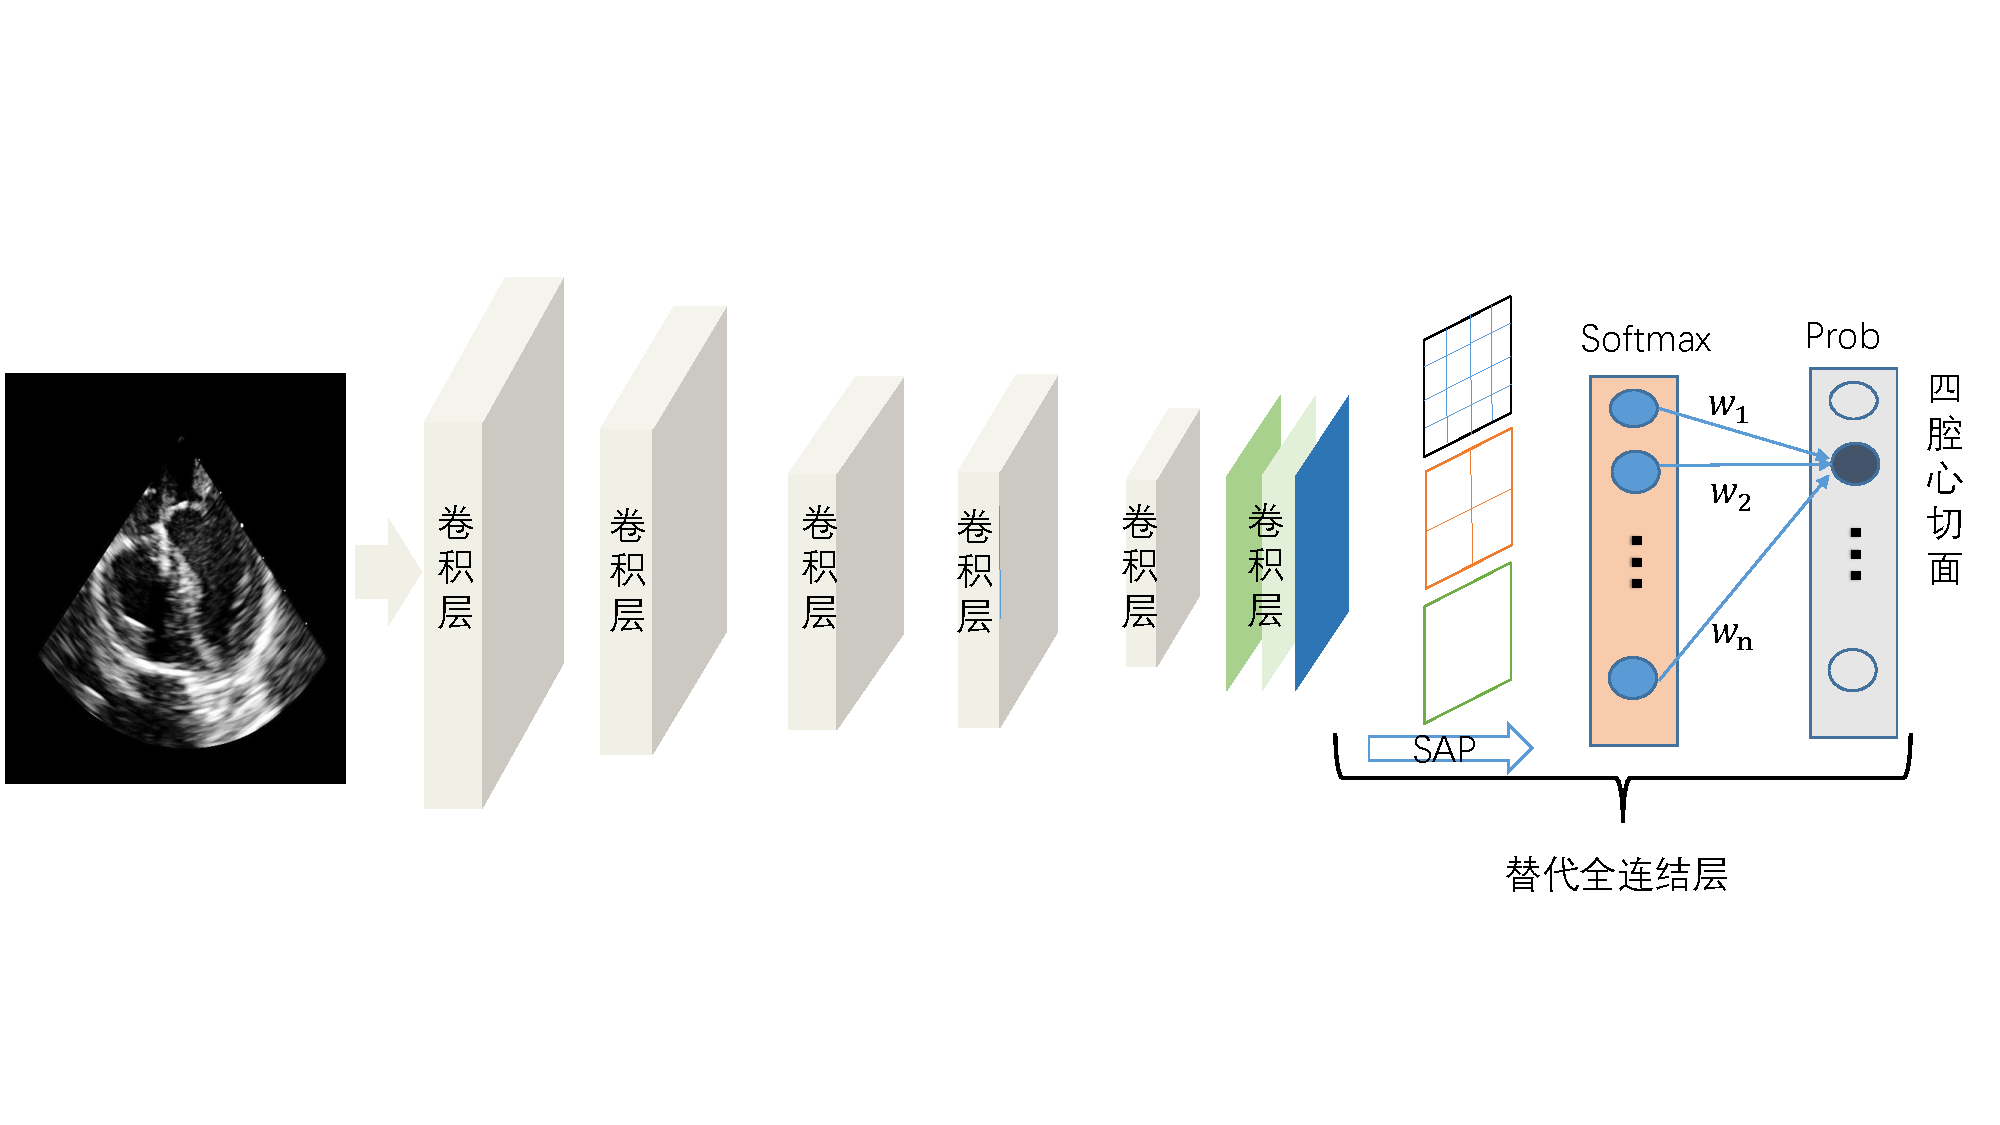
\includegraphics[trim = 30mm 0mm 30mm 0mm, clip, width=0.45\textwidth]{ch03_02}
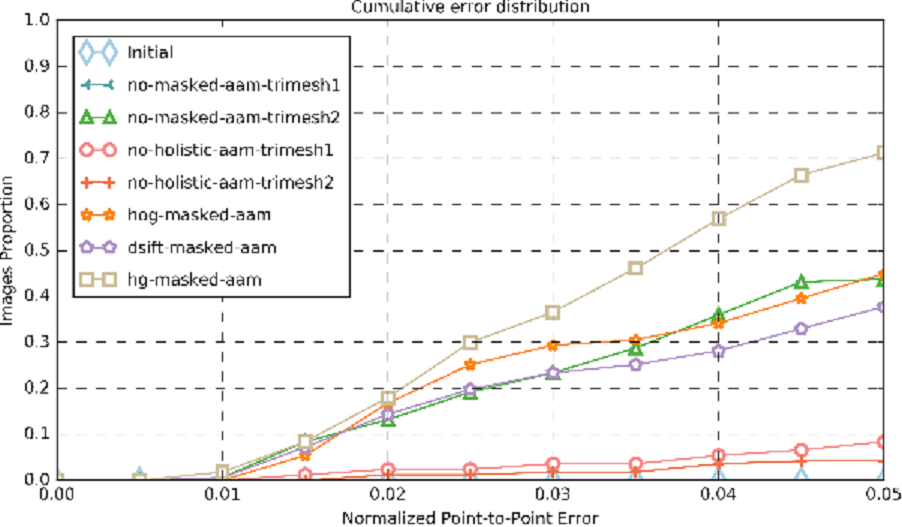
\includegraphics[width=0.85\textwidth]{ch07_05}
\caption{不同特征AAM的左心室内外膜分割性能比较}
\label{fig:ch07_05}
\end{figure}  

公式1中外观纹理的对齐较大程度上依赖三角网格的划分,与人脸对齐的差异是,心室分割中的三角网格并不总是都有一定实际意义,本文对比实验了两种的三角网格(图1c,3b)。同时由于心外膜周围区域较难定义特征点及定位,实验发现基于块的全局AAM(图3c和图5中masked)普遍优与全局AAM(图5中holistic)的方法。
\begin{figure}[!htbp]
\centering
%trim option's parameter order: left bottom right top
%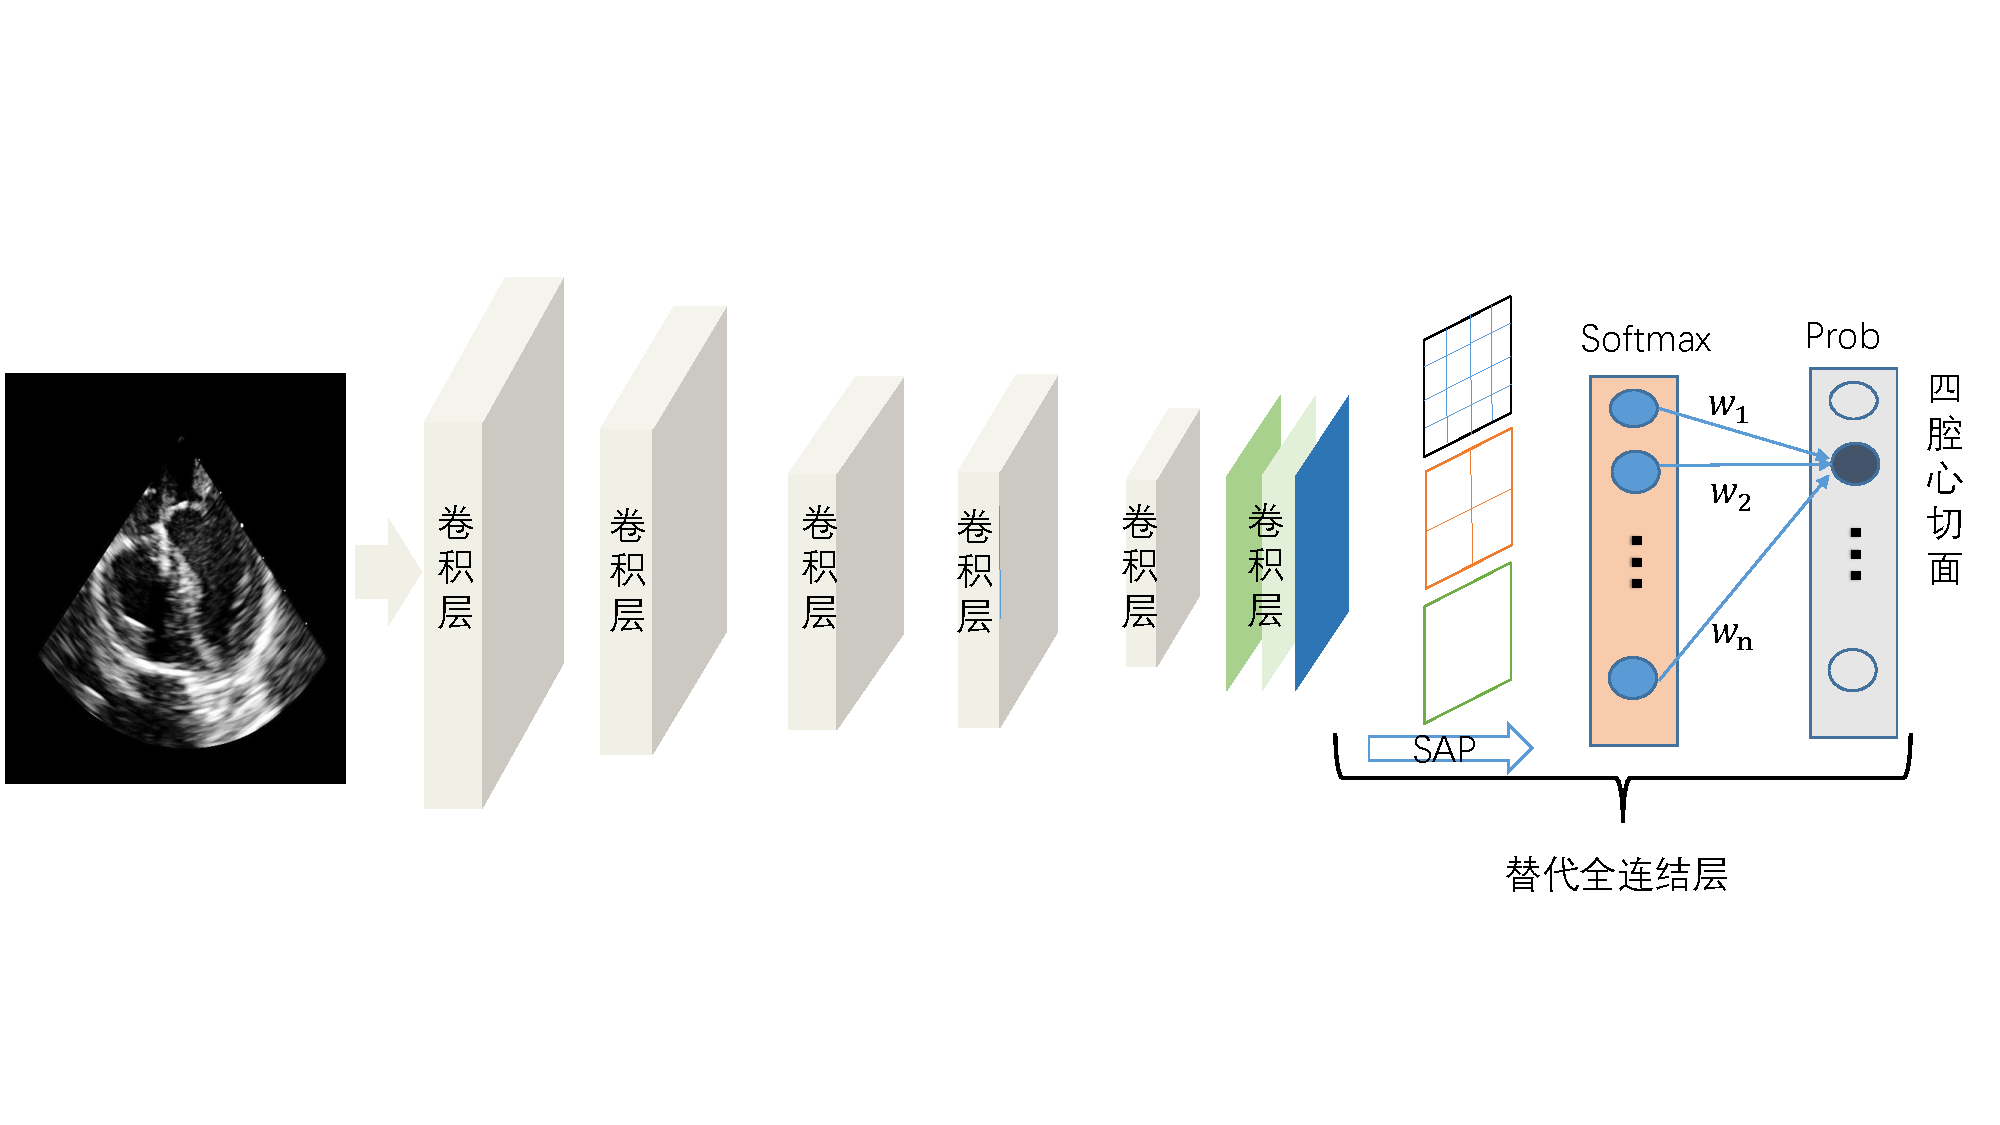
\includegraphics[trim = 30mm 0mm 30mm 0mm, clip, width=0.45\textwidth]{ch03_02}
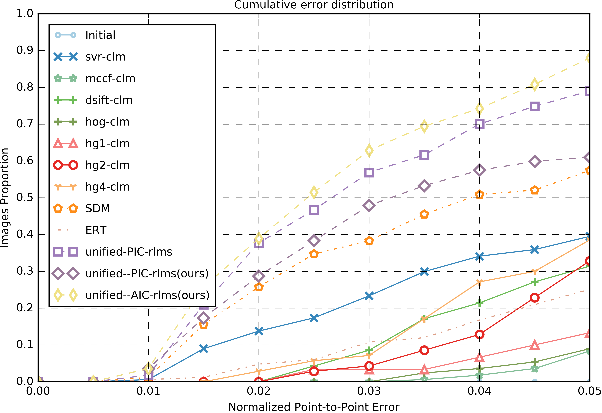
\includegraphics[width=0.85\textwidth]{ch07_06}
\caption{分割结果对比}
\label{fig:ch07_06}
\end{figure}  
 
 
分割性能见图\ref{fig:ch07_05},外观特征比较了原始像素(no)、dsift\citep{Lowe2004}、HOG和HG特征,结果表明采用HG网络自动特征的分割效果远优于手工设计的特征(图\ref{fig:ch07_05}中hg-masked-aam),其中dsift(8个通道)和hog(32个通道)效果比只使用灰度的结果要好;实验结果表明只使用原始像素,
即使用第3.1节提出的超声组织特征纹理特异性灰度归一化,得到的形状无关的外观纹理(图\ref{fig:ch07_03}b)与真实心动图差异仍较大,导致分割效果较差(图\ref{fig:ch07_05}中no曲线 ),主要原因是因为AAM方法对初始值敏感,之前文献\citep{Bosch2002,Hansson2014}中实验验证时仅是根据真实形状施加噪声扰动作为初始值\citep{jixianghu-2016},这不符合实际情况,本文提出心室检测作为初始轮廓的放置依据。

基于不同特征的CLM分割效果如图6所示,CLM方法相比AAM方法的分割结果较差,主要是由于针对超声图像的分割极易陷入局部极值,无论是基于判别分类SVR还是基于概率生成MCCF的CLM模型分割结果都较差,即使结合HG特征改进效果也不明显,这主要是因为HG网络是基于特征点周围服从高斯分布的假设训练得到,这对超声心动图明显不十分合适,这也是下一步需要改进的方面。而随着层级的加大得到更多的全局信息,CLM分割效果逐渐提升(图6中hg1,2,4),但仍劣于基于判别分类回归的SVR方法。
\subsection{结合最优的AAM和CLM分割结果}
结合前文提出基于4级HG网络特征的AAM和CLM模型,克服两者相应缺点,能得到本文的最优结果(图\ref{fig:ch07_06}中unified-PIC-rlms表示采用文献\citep{Jan2017}提出的方法),其中PIC和AIC分别表示前文提到对AAM模型两种迭代算法,rlms表示对CLM模型的优化方法。同时跟基于级联形状回归的ert算法\citep{Kazemi2014a}和sdm算法\citep{Xiong2013}进行实验比较,相应实验参数设置同原论文,结果表明提出方法的结果的有效性。

\begin{table}[!htbp]
    \centering
    \footnotesize% fontsize
    \setlength{\tabcolsep}{4pt}% column separation
    \renewcommand{\arraystretch}{1.2}%row space 
    \begin{tabular}{lcccccc}
        \cline{1-7}% partial hline from column i to column j
         方法  &A  &B &C1 &C2	&C3	&C4 \\
        \hline
        均值	&59.5	&72.7	&54.8	&57.2	&55.6	&57.8 \\
        \hline
        方差	&21.4	&25.2	&21.8	&20.7	&21.5	&20.3\\
        \hline\hline
    \end{tabular}
    \caption{不同分割方法与专家标注的对比统计}
    \label{tab:ch07_01}
\end{table}

计算预测形状与专家标注形状之间的距离,然后统计这些距离的均值和方差,得到的统计结果见表\ref{tab:ch07_01}。表中A代表结合4级HG特征的AAM(错误率阈值为0.03);B代表结合4级HG特征的CLM方法;用统一AAM和CLM结合4级HG特征表示本方法,C1代表本方法下错误率阈值为0.05的内膜分割结果;C2代表本方法下错误率阈值为0.05的外膜分割结果;C3代表本方法下错误率阈值为0.02的内膜分割结果;C4代表本方法下错误率阈值为0.02的外膜分割结果。结果表明从总体形状间的平均距离上能看提出内膜分割明显优于外膜分割结果,验证方法的有效性(表\ref{tab:ch07_01})。由图\ref{fig:ch07_07}a中可见,本文方法结果与专家标注比较接近。
\begin{figure}[!htbp]
\centering
%trim option's parameter order: left bottom right top
%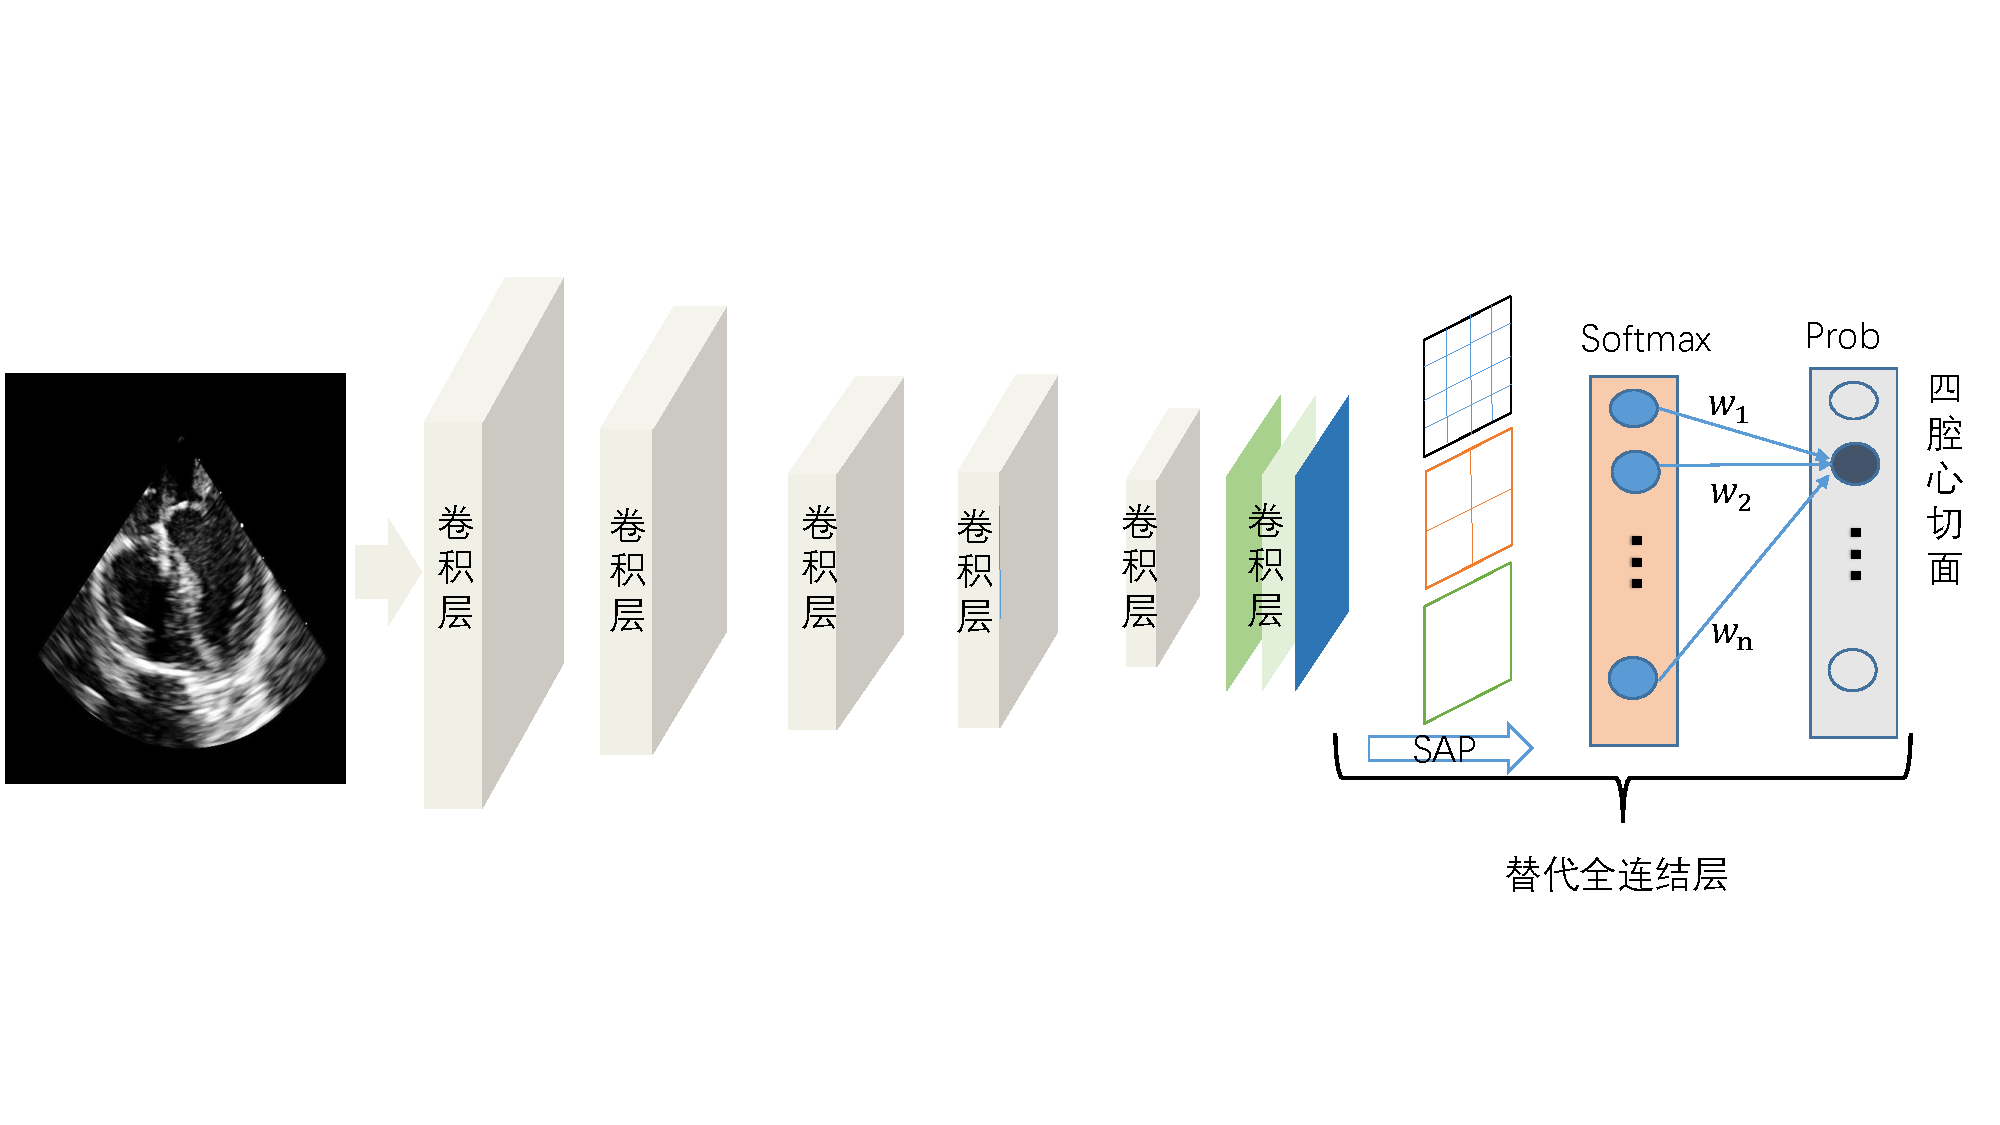
\includegraphics[trim = 30mm 0mm 30mm 0mm, clip, width=0.45\textwidth]{ch03_02}
\includegraphics[width=0.85\textwidth]{ch07_07}
\caption{用HG网络预测心室内外膜成功和失败的案例}
\label{fig:ch07_07}
\end{figure}   

从分割失败的案例中能得知,尽管基于HG网络能综合建模心室外观的全局和局部特征,且该特征确实是对内外膜的响应(图\ref{fig:ch07_07}c),但由于特征点之间并没有形状和顺序信息,有可能导致分割失败。

\section{小结与讨论}

本文提出了一种基于沙漏卷积神经网络特征的统计形状模型分割方法,针对医学图像的组织分割任务,在自动检测左心室提供初始化轮廓的基础上,通过统一全局AAM和CLM模型的概率解释,综合两种方法的优点自动同时分割左心室内膜和外膜。在心室分割数据集上的实验结果表明,本文提出的自动分割方法在准确度和可解释性方面优于许多已有的分割方法.因此,本文的方法是可行的和有效的。

